% A 差异与收束约 2 分钟；放在 B、C 讲解之后。
\begin{frame}{条件差异：比较结构内部的相对强度}
\textbf{344 个结构 $\times$ 2 个突变条件 = 688 行比较。}
\vspace{0.4em}

同一区间取六样本共同有效像素；条件内先平均两个重复，再与 WT 比较。
\[
F_c=\log_2\frac{\overline S_c}{\overline S_{\mathrm{WT}}},\qquad
b=\max\!\left(\log_2 1.25,\left|\log_2\frac{S_{\mathrm{WT},2}}{S_{\mathrm{WT},1}}\right|\right)
\]
\small 两个突变重复都越过同一侧参照带才标为一致增强或减弱。
\vspace{0.7em}

\centering
\begin{tabular}{lrrrr}
\toprule
条件 & 增强 & 减弱 & 带内 & 边界/不一致 \\
\midrule
$\Delta stpA$ & 217 & 6 & 94 & 27 \\
$\Delta hns\Delta stpA$ & 182 & 10 & 92 & 60 \\
\bottomrule
\end{tabular}
\vspace{0.6em}

\raggedright\small 描述性参照，不是显著性检验；12 个低覆盖结构留在全表，不用于代表案例。
\end{frame}

\begin{frame}{实例：CHIN\_126 在 $\Delta stpA$ 下重复一致增强}
\centering
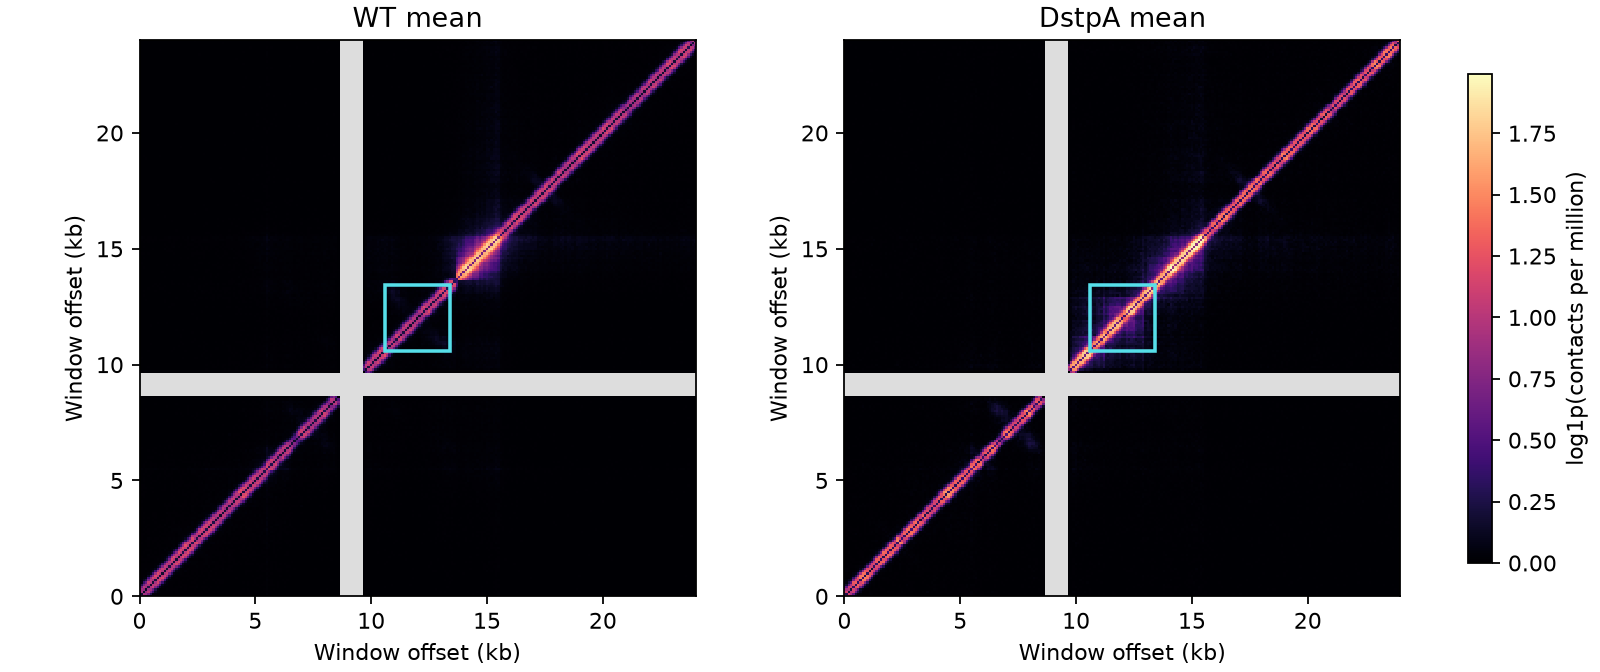
\includegraphics[width=0.94\textwidth]{../results/differences/figures/CHIN_126_DstpA_slide.png}\\[0.3em]
\small 青框为量化区间；灰色为共同无效区域。均值约为 WT 的 \textbf{2.504 倍}。\\[0.4em]
\small 两重复相对 WT 的 $\log_2$ 比为 1.306、1.342，均高于参照带上界 0.322。
\end{frame}

\begin{frame}{结论与解释范围}
\begin{block}{已完成的比较}
\normalsize 共享流程连接分类、候选发现、465 张轨道图及 688 行条件比较。\\
同一条件下既有增强也有减弱，代表案例同时保留稳定与边界结果。
\end{block}
\vspace{0.5em}
\begin{itemize}
\item 47 个高分候选仅对应 10 个独立位置；目前没有满足规则的疑似新簇。
\item 深度归一化后的相对增强，不等于细胞内绝对接触总量增加。
\item 两个重复用于描述性对照，双缺失结果不归因于单个因子。
\end{itemize}
\vspace{0.6em}
\small\textcolor{projectblue}{阶段稿：最终录制前，在 B 的章节补齐分类测试、基线/解释图与跨重复验证结论。}
\end{frame}
